\documentclass{beamer}
\setbeamertemplate{section in toc}[circle]
\setbeamertemplate{subsection in toc}[circle]

\title{Logiciel de compression}
\subtitle{Programmation Impérative III}
\author{Tom YUNGMANN, Adrian AUBE}
\institute{Faculté des Sciences et Techniques, Université Jean Monnet}
\date{2024}

\begin{document}

\frame{\titlepage}

\begin{frame}{Table des matières}
    \tableofcontents
\end{frame}



\section{Compression et décompression}

\subsection{Un fichier}

\begin{frame}{Format du fichier compressé}
    
\includegraphics[scale=0.3]{latex_alphabet.png}
    
\includegraphics[scale=0.24]{latex_separator.png} 
    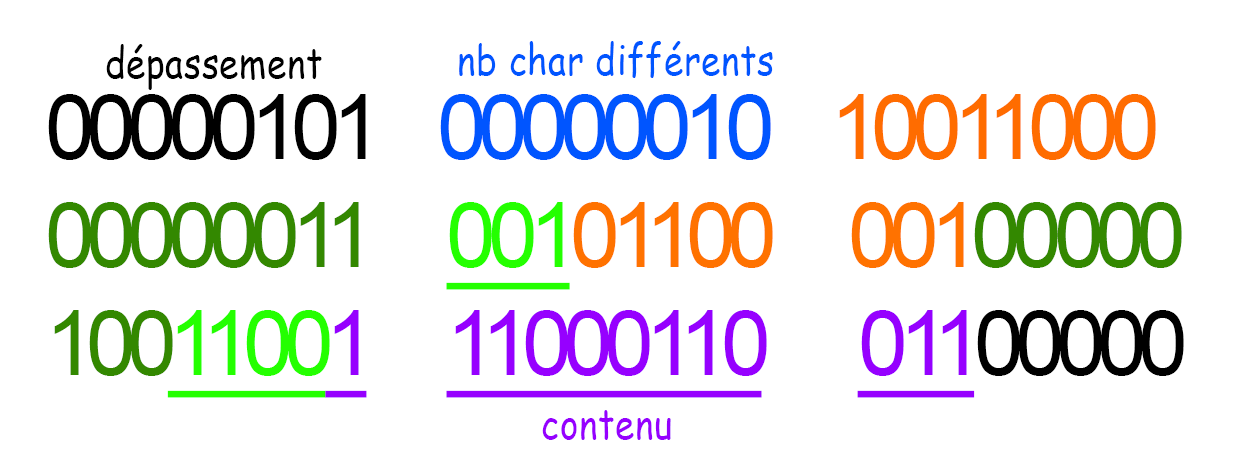
\includegraphics[scale=0.24]{latex_1seulfichier.png} 
\end{frame}

\subsection{Plusieurs fichiers ou dossiers}

\begin{frame}{Plusieurs fichiers ou dossiers}
    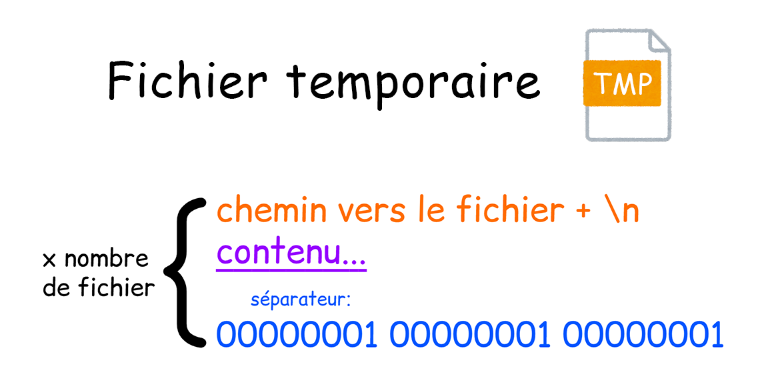
\includegraphics[scale=0.5]{latex_tmp.png}
\end{frame}

\begin{frame}{Plusieurs fichiers ou dossiers}
    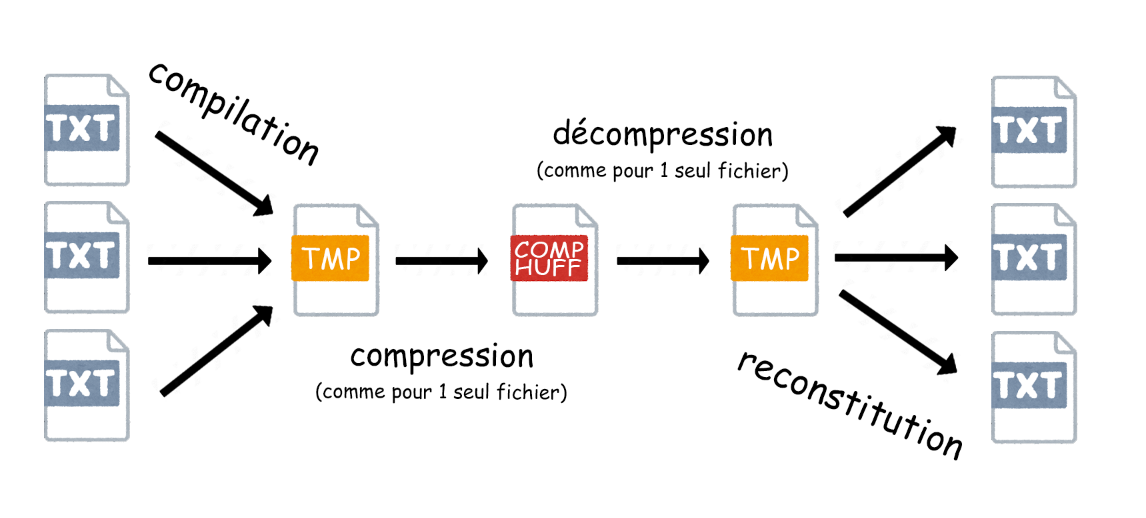
\includegraphics[scale=0.37]{latex_multifichier.png}
\end{frame}



\section{Étude du taux de compression}

\subsection{Fichier unique}

\subsubsection{Taille du fichier}
\begin{frame}{Taille du fichier}
    Paramètres fix : 32 caractères différents de même fréquence
    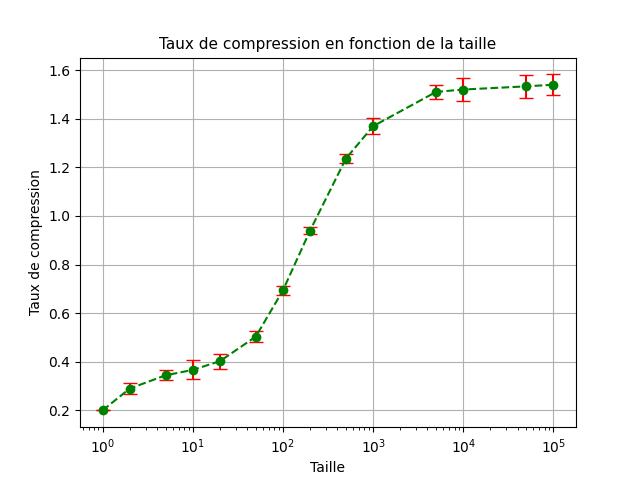
\includegraphics[scale=0.66]{taille.png}
\end{frame}

\subsubsection{Nombre de caractères différents}
\begin{frame}{Nombre de caractères différents}
    Paramètres fix : 10 000 caractères de même fréquence
    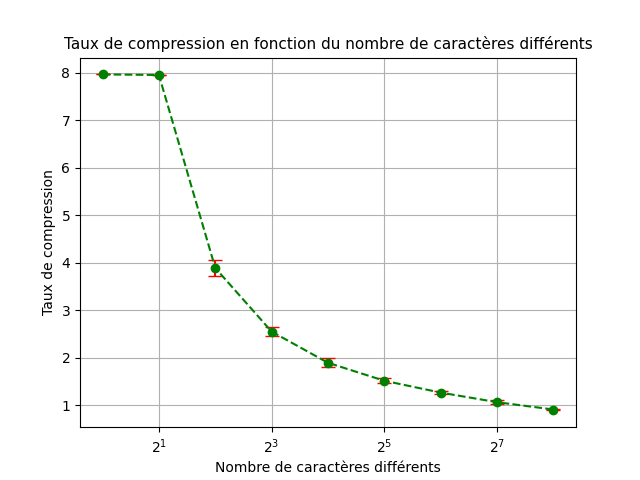
\includegraphics[scale=0.66]{car_diff.png}
\end{frame}

\subsubsection{Fréquence des caractères}
\begin{frame}{Fréquence des caractères}
    Paramètres fix : 10 000 caractères, 8 différents
    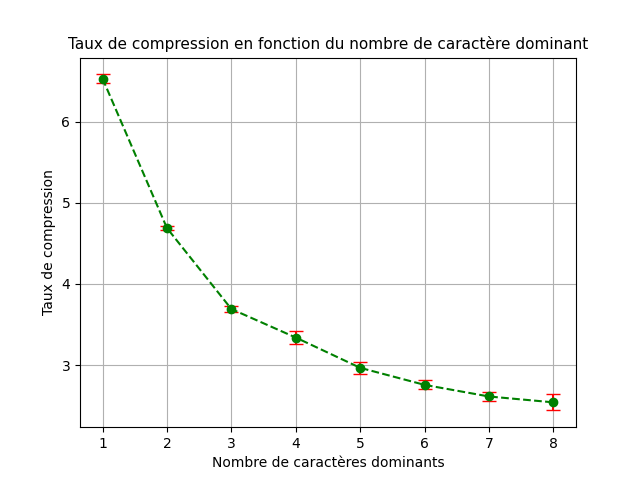
\includegraphics[scale=0.66]{freq_dom.png}
\end{frame}
\begin{frame}{Fréquence des caractères}
    Paramètres fix : 10 000 caractères, 8 différents
    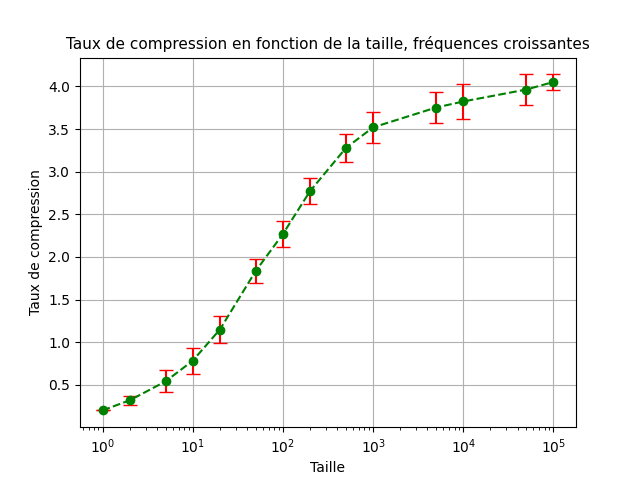
\includegraphics[scale=0.66]{freq_croiss.png}
\end{frame}

\subsection{Plusieurs fichiers}
\begin{frame}{Plusieurs fichiers}
    Paramètres fix : 1 000 caractères, 64 différents de même fréquence, nom du fichier sur maximum 3 chiffres
    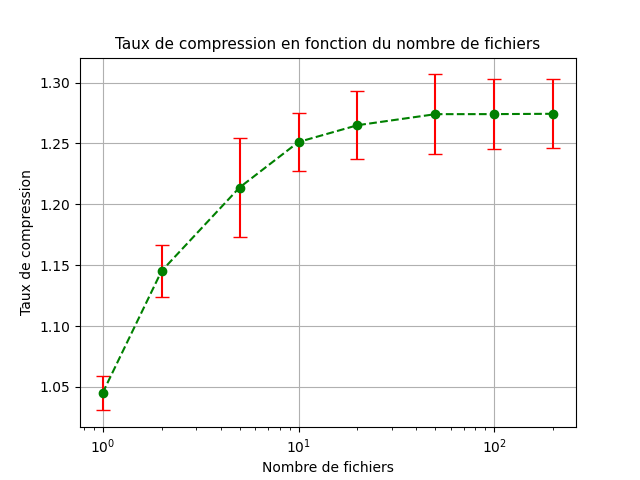
\includegraphics[scale=0.6]{nb_fich.png}
\end{frame}

\begin{frame}{Dossiers imbriqués}
    Paramètres fix : 1 fichier par dossier de taille 1 000, 32 caractères différents de même fréquence, nom : "0". Nom des dossiers : numéro sur maximum 2 chiffres 
    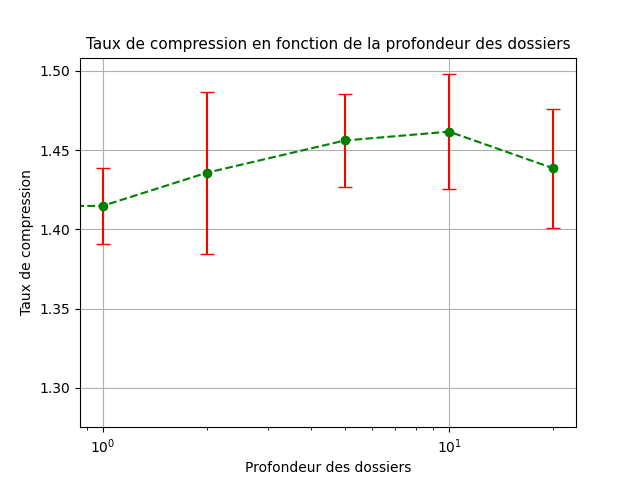
\includegraphics[scale=0.57]{prof_doss.png}
\end{frame}

\end{document}
